\section{Energy Compact Model}
\subsection{Renewable Energy Usage Targets}Based on our discussion in Evaluation Criteria for the best Profile and above models, the average price of electricity in 2025 and 2050 respectively.\\
\autoref{predic} presents the predictive values of average price in 2025 and 2050. Find the average price of the four states in 2025 and 2050 are 35.32732299 and 43.71283002 based on the fit curves as shown in \autoref{fig:AvePrice}\\

Therefore, the average price of the four states in 2025 should be set at about 28.26(80\% of the predictive values absent any policy changes) dollars.\\
In 2050 the average price should be set at about 34.97(80\% of the predictive values absent any policy changes) dollars. We state it as the goal for this new four-state energy compact.\\ In order to establish Interstate Energy Price Contract for 2025 and 2050, we obtain the table by using the above two models, that is, Growth Rate Model and Energy Proportion Model. We predict the total consumption and the proportion of renewable energy in 2025 and 2050 from two kinds of ideas. It can be seen in \autoref{error} that the two models have small error of the simulation. The fact indicates that the two models are successful.\\
\begin{table}[h]
	\centering
	\caption{The predictive Values of average Price in 2025 and 2050}
	\label{predic}
	\begin{tabular}{|c|c|c|c|c|}
		\hline
		& AZ          & CA          & NM          & TX          \\ \hline
		2025 & 39.62902025 & 36.22521619 & 34.23589234 & 31.21916318 \\ \hline
		2050 & 43.44450209 & 42.34353690 & 45.45793568 & 43.60534539 \\ \hline
	\end{tabular}
\end{table}
\begin{figure}[h]
	\centering                                             %居中
	\subfigure[Average Price of AZ]{                    %第一张子图
		\begin{minipage}{7cm}
			\centering                         %子图居中
			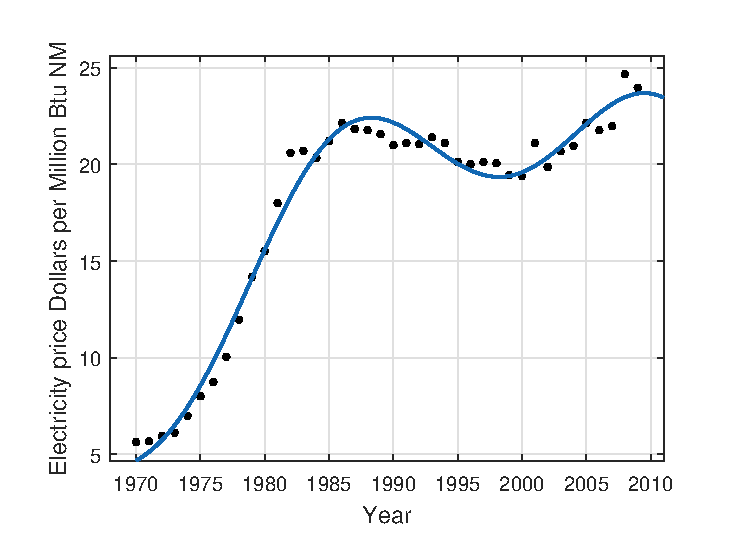
\includegraphics[scale=0.5]{figure/junjiaAZ}    %以pic.jpg的0.5倍大小输出
	\end{minipage}}
	\subfigure[Average Price of CA ]{                    %第二张子图
		\begin{minipage}{7cm}
			\centering                                     %子图居中
			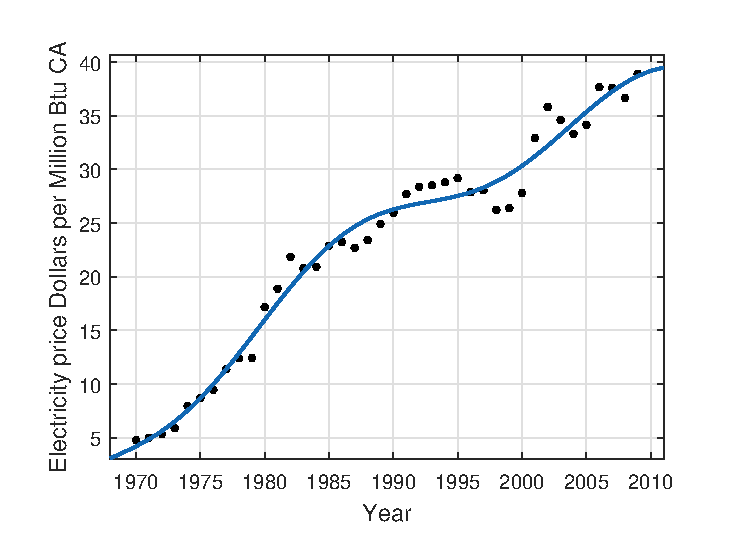
\includegraphics[scale=0.5]{figure/junjiaCA}      %以pic.jpg的0.5倍大小输出
	\end{minipage}}
	\subfigure[Average Price of NM]{                    %第三张子图
		\begin{minipage}{7cm}
			\centering                         %子图居中
			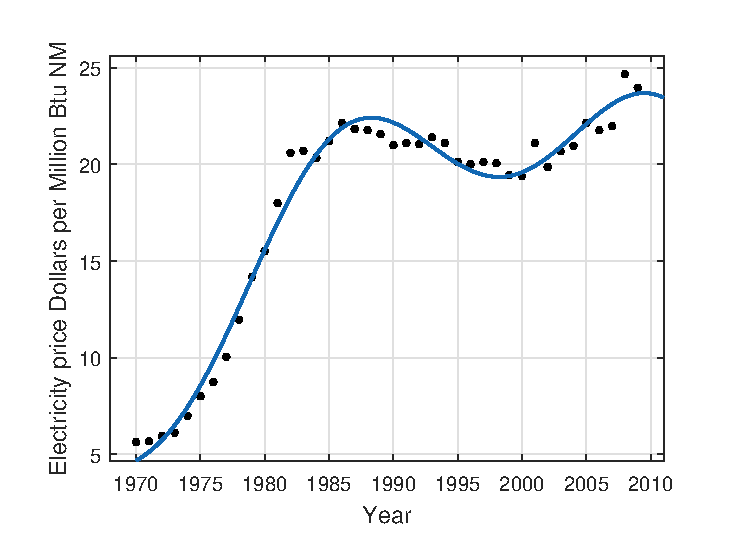
\includegraphics[scale=0.5]{figure/junjiaNM}    %以pic.jpg的0.5倍大小输出
	\end{minipage}}
	\subfigure[Average Price of TX]{                    %第四张子图
		\begin{minipage}{7cm}
			\centering                                     %子图居中
			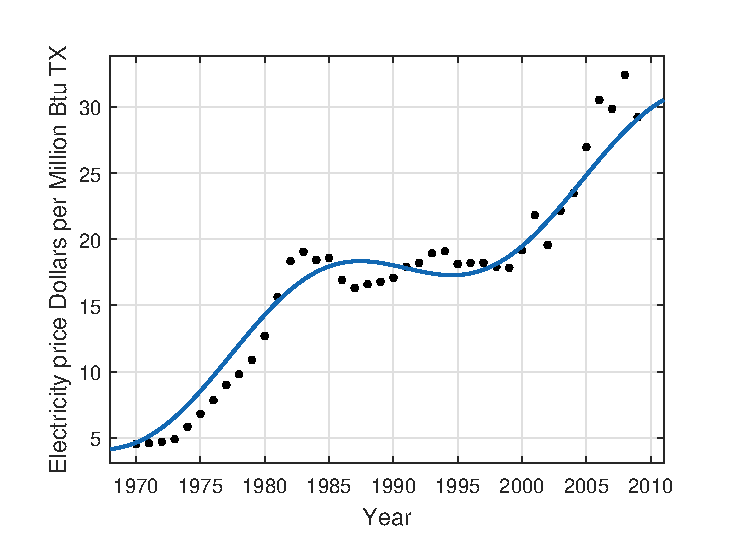
\includegraphics[scale=0.5]{figure/junjiaTX}      %以pic.jpg的0.5倍大小输出
	\end{minipage}}
	\caption{Four-State Average Price of Recreatable Energy over time}                      %大图名称
	\label{fig:AvePrice}                                       %图片引用标记
\end{figure}
\begin{table}[h]
	\centering
	\caption{The error between the two model predictive values}
	\label{error}
	\begin{tabular}{|l|l|l|l|l|l|}
		\hline
		& Predictive value                & AZ      & CA      & NM      & TX      \\ \hline
		\multirow{3}{*}{2025} & Proportion predicted by the proportion & 9.45\%  & 10.12\% & 8.43\%  & 6.21\%  \\ \cline{2-6} 
		& Proportion predicted by growth rate& 9.55\%  & 12\%    & 9.31\%  & 6.65\%  \\ \cline{2-6} 
		& error                           & -0.10\% & -1.54\% & -0.88\% & -0.45\% \\ \hline
		\multirow{3}{*}{2050} & Proportion predicted by the proportion  & 33.19\% & 15.76\% & 10.79\% & 9.82\%  \\ \cline{2-6} 
		& Proportion predicted by growth rate& 9.73\%  & 17.27\% & 10.11\% & 8\%     \\ \cline{2-6} 
		& Error                           & 23.46\% & -1.51\% & 0.68\%  & 5.00\%  \\ \hline
	\end{tabular}
\end{table}
\subsection{Actions to meet the Energy Compact Goal}
\begin{itemize}
	\item Support clean coal technology.\\ According to our prediction model, the future fossil energy consumption of the United States is still very large, and the proportion of the total energy consumption is also large.  Therefore, in order to achieve the goal of the Western Interstate Energy Compact, namely to increase amount of usage of renewable energy and utilization ratio, states have to reduce the proportion of fossil fuel and increase the efficiency of usage of fossil fuels. Supporting clean coal technology can improve coal utilization and heat conversion efficiency. Such measures could effectively reduce fossil fuel's consumption.
	\item Support photovoltaic solar cell semiconductor materials research.\\ Since the U.S. will adopt a new energy plan, it will inevitably slow the development of renewable energy, which will have a negative impact on global climate change. Most of renewable energy production will not have a larger effect on the environment (except hydroelectricity industry), so continue to support the development of renewable energy is indispensable. However, most renewable energy depends on the natural conditions. Increasing the energy conversion rate of photovoltaic solar energy and reducing the cost of photovoltaic solar energy generation can make the production of this renewable energy source as environmentally-friendly as possible.
	\item Apply preferential policies to energy transactions between the states.\\ Lower the threshold of energy trade across the states, and strengthen the interstate commerce energy flow. In order to realize the Western Interstate Energy Contract and promote the cooperation among the states, states should reach an agreement on the interstate commerce of energy. States also should adopt preferential policies to deal with the interstate energy trade, especially the electricity trade generated from renewable energy production. And states should gradually coordinate their distributionof the renewable energy industry with other states according to their own geographical conditions and industrial needs. So that state's renewable energy efficiency ratio will be as low as possible.
\end{itemize}

